\section{实验内容\cite{pcl2002}}

\subsection{仪器与药品}

不同浓度的正丁醇水溶液(不同浓度的正丁醇溶液 ($0.0218 \mathrm{~mol} / \mathrm{L}, 0.0547 \mathrm{~mol} / \mathrm{L}, 0.111 \mathrm{~mol} / \mathrm{L}, 0.220 \mathrm{~mol} / \mathrm{L}$, $0.329 \mathrm{~mol} / \mathrm{L}, 0.439 \mathrm{~mol} / \mathrm{L}, 0.550 \mathrm{~mol} / \mathrm{L}, 0.740 \mathrm{~mol} / \mathrm{L}$)。

最大气泡压力法表面张力测量装置, QBZY-2 型表面张力仪。

\subsection{实验步骤与条件}

\begin{figure}[H]
    \centering
    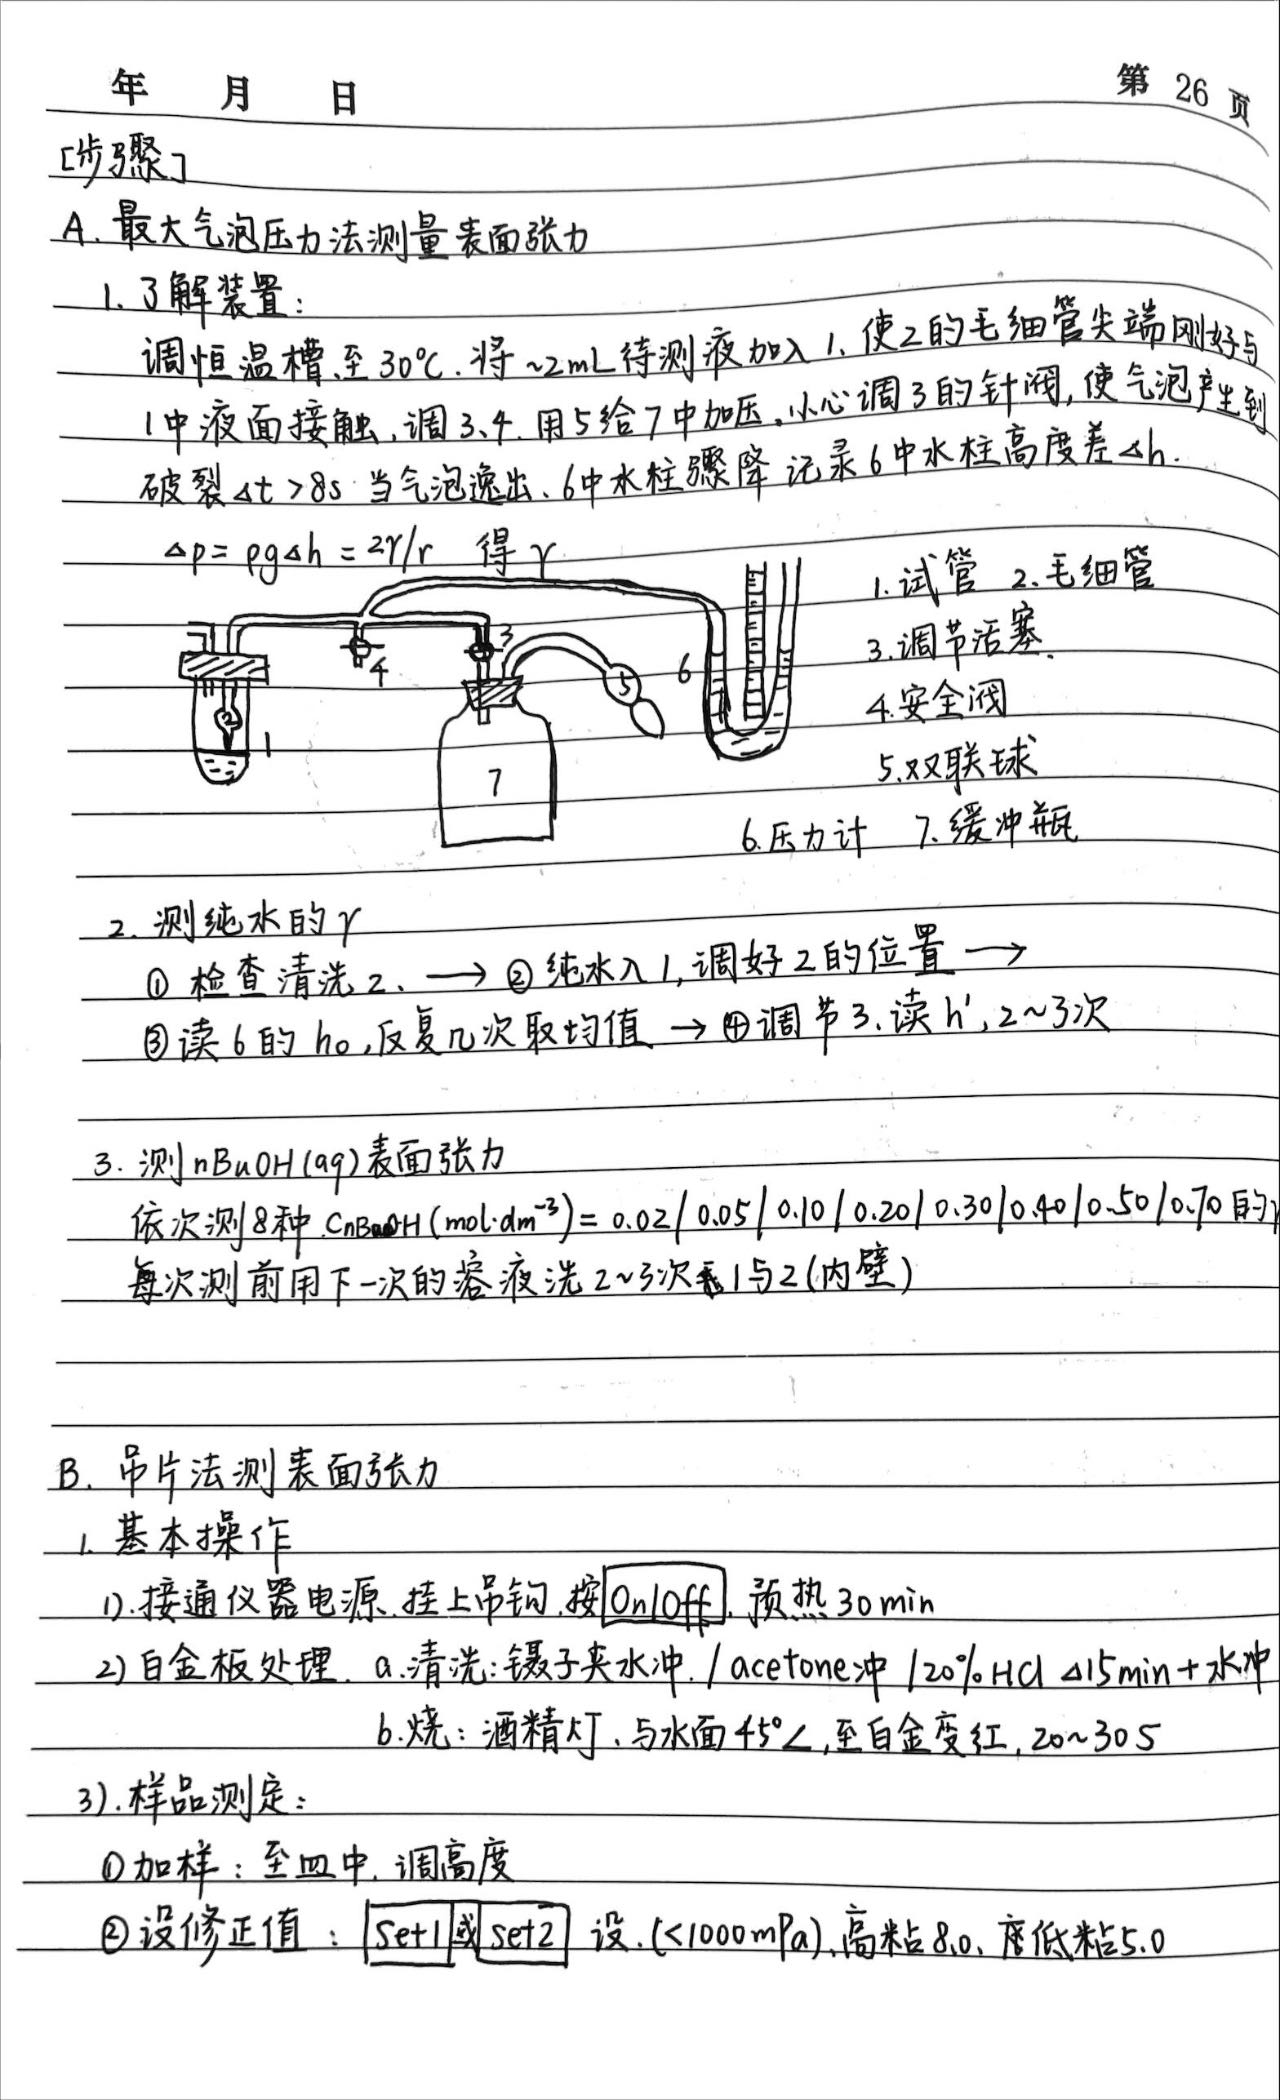
\includegraphics[width=.7\textwidth]{figures/0-3.jpg}
    \bicaption{预习报告:实验步骤与条件(1)}{Preview report: steps and conditions No.1 of the experiment}
\end{figure}

\begin{figure}[H]
    \centering
    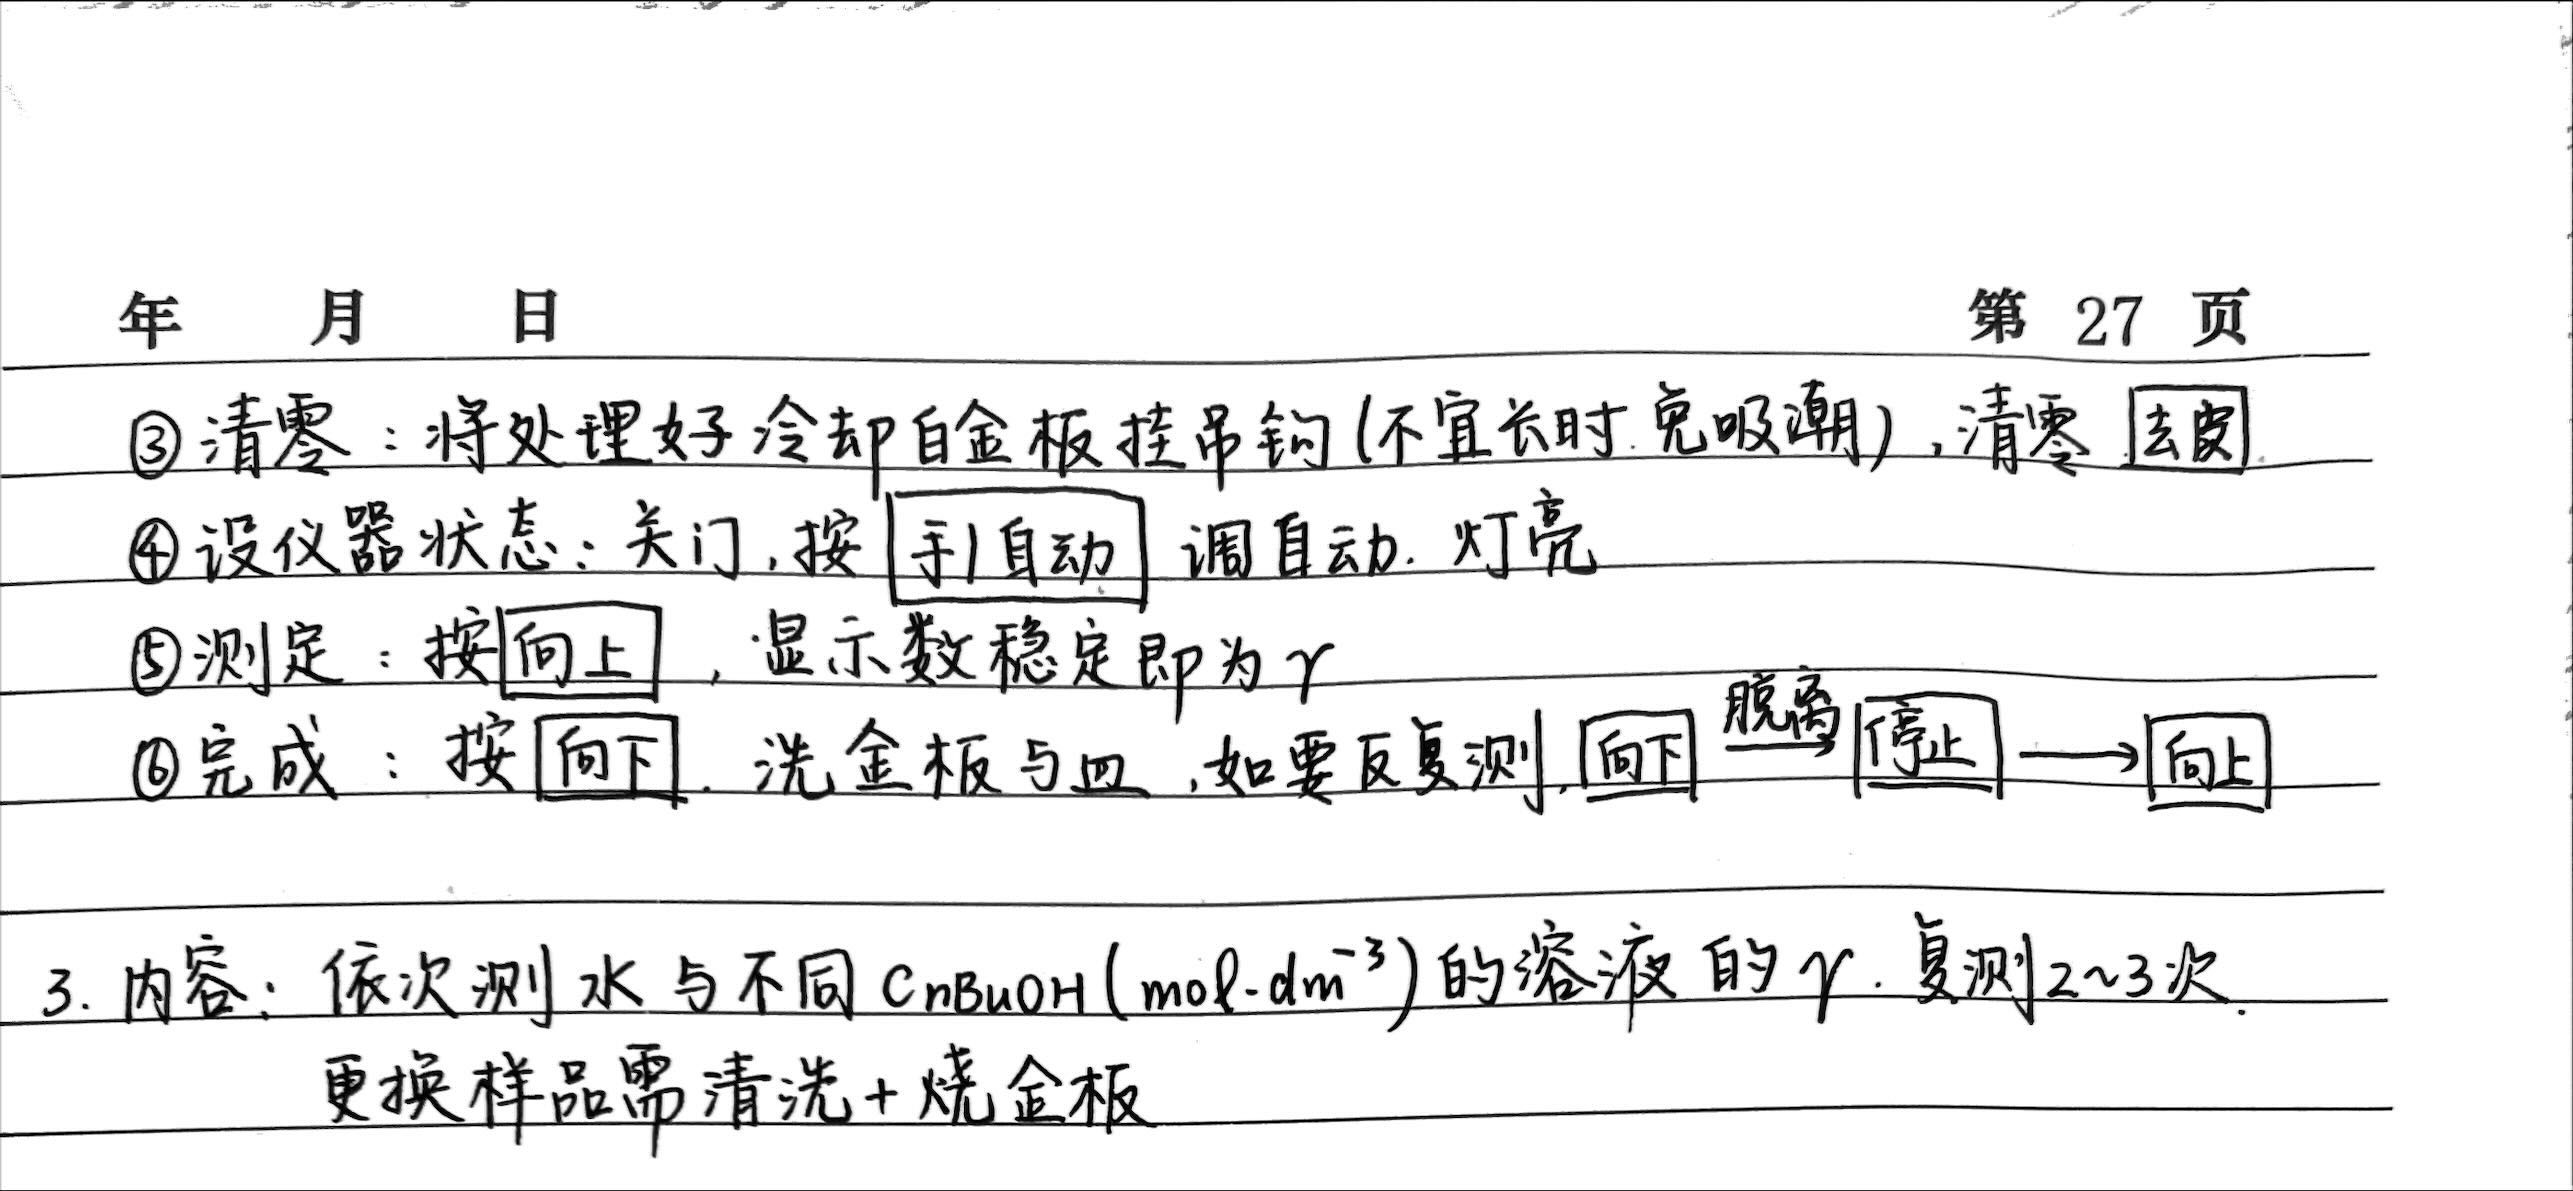
\includegraphics[width=.7\textwidth]{figures/0-4.jpg}
    \bicaption{预习报告:实验步骤与条件(2)}{Preview report: steps and conditions No.2 of the experiment}
\end{figure}
